%===================================== CHAP 3 =================================

\chapter{Methods and implementation}\label{chpt:methods}

\section{Programming environment}

Theano is a Python library for building high-performance mathematical tools \citep{Bergstra2010}. It lets you write library-specific code which will be analyzed, optimized, and compiled to C or CUDA, enabling execution of efficient bytecode. Furthermore, Theano lets you symbolically define an algorithm in a high-level programming environment. For those familiar with Mathematica, symbolic definition in Theano is fairly similar. In this thesis Python and Theano is used for model implementation, the experiments being outlined in chapter \ref{chpt:experiments}.

Theano is tightly integrated with NumPy, another Python package for scientific computation. Moreover, Theano supports parsing of several NumPy objects into objects which Theano will be able to later use efficiently after its optimization process. Please consult LISA lab's webpage \citep{LISA-lab2015a} for a complete documentation of the framework.
Theano operates on symbolic constructs, called tensors; general mathematical constructs. So in order to define a function, you would write the actual mathematical expression, for instance:

\begin{verbatim}
import theano.tensor as T
import theano

A = T.fmatrix('A')
y = A ** 2
f = theano.function([A], y)
\end{verbatim}

Calling the library function theano.function analyses the symbolic expression, and constructs executable C or CUDA code from it. See Appendix C for a slightly more advanced example using the scan-operator in theano.

When defining symbolic expressions such as functions using Theano, Theano constructs a graph of the provided symbolic expressions, see figure \ref{fig:theano_graph_demo}. This allows for differentiation and manipulation through a syntactic and semantic analysis of the resulting expression graph, optimizing the graph for expression evaluation and graph traversal before code generation. The compiler may then generate optimized code, compiling it according to the provided environmental parameters. This leads to highly efficient C or CUDA executable code.
Note, however, that as the library provides a high-level abstraction for generation of efficient C or CUDA-code, this renders debugging somewhat harder. More specifically, the executable code will be further processed from that in Python and Theano. This means that the programmer may need to predict more about how the code will be compiled, making it highly recommendable or necessary to have some previous knowledge within C and/or how the Python-library's compilation process works. A remedy for this is howeevr that Theano supports profiling, providing the programmer with information about what data structures the variables are compiled to, as well information about as their usage. Furthermore, if compiling to a GPU, Theano may output warnings whenever an operation is performed on the CPU.

\begin{figure}
\centering
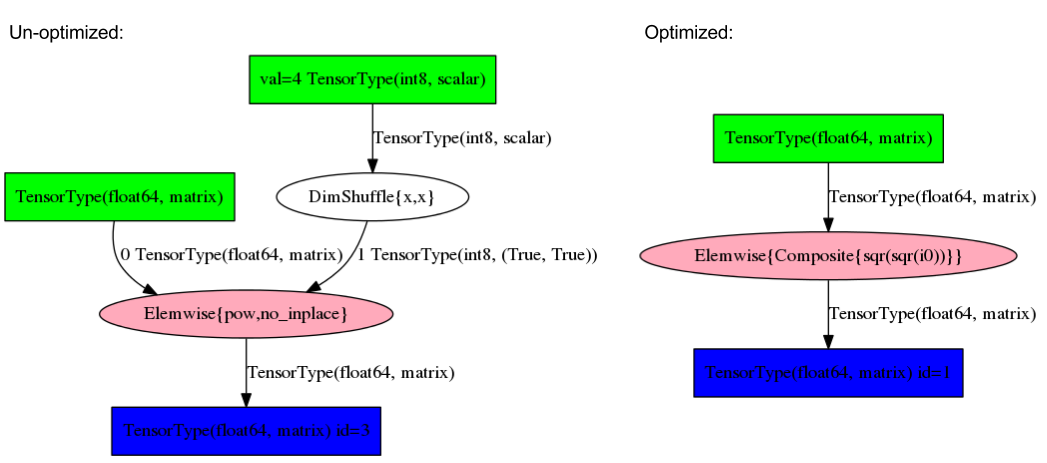
\includegraphics[width=12cm]{fig/unopt_opt_theano_graph}
\caption{Graph manipulation of tensors in Theano during the optimization and compilation process of an expression such as $y = A^2$.}
\label{fig:theano_graph_demo}
\end{figure}

In order to use Theano, certain dependencies need to be setup. These are fairly straightforward when it comes to compiling to C-code for CPU-execution. In a preliminary study for this thesis, I setup Theano for use with a GPU on a system with an NVIDIA card, using Ubuntu 14.04 LTS. I consulted the guide found on \citep{LISA-lab2015b} to obtain installation instructions for doing so. In doing so I found that kWTA requires the dual-network memory model to be synchronized, thus requiring transferring control to the CPU and interpreter, including memory transfer from the GPU to the CPU. Therefore, running the model on the GPU did not provide for any substantial run-time performance gain for the HPC-network. Therefore I decided to target the CPU, particularly when it comes to the HPC-module, which may only be executed on the CPU in its current form. Running only the neocortical network on a data-set would, however, be far more efficient using the GPU. In fact, the compiler may target the GPU if the framework for it is setup, and the Theano flags allows a hybrid approach (i.e. no device parameters are set).

% ========================================== SYSTEM ================================================
\subsection{System layout}

The dual-network memory model is implemented using Python and the library Theano, as described above. In order to instantiate the model, test it, run experiments, and store results; I developed a complete framework within Python in order to do so. The core components of the system are the classes HPC and NeocorticalNetwork. These contain all methods associated with the hippocampal and neocortical network, that are required to perform the algorithmic operations of the dual-network system as outlined in \citep{Hattori2014}. Furthermore, these core classes make use of certain static functions such as displaying a visualization of the current network output during run-time, or writing to a log. These were defined in a Tools-package. In order to verify the functionality of the core modules, I wrote a small test suite, using 'unittest', that may be used to automate debugging processes. Furthermore, I wrote a hippocampal module wrapper implementing an abstraction of learning a set of patterns using a hpc-model, performing chaotic recall for a given model and object instance, and generation of pseudopatterns of class II for a given set of chaotically extracted patterns as well of parameters specifying the pseudopattern generation preferences. This wrapper is used in the experimental suite, which implements the experiments that are outlined in the following chapter (\ref{chpt:experiments}).

\begin{figure}
    \centering
    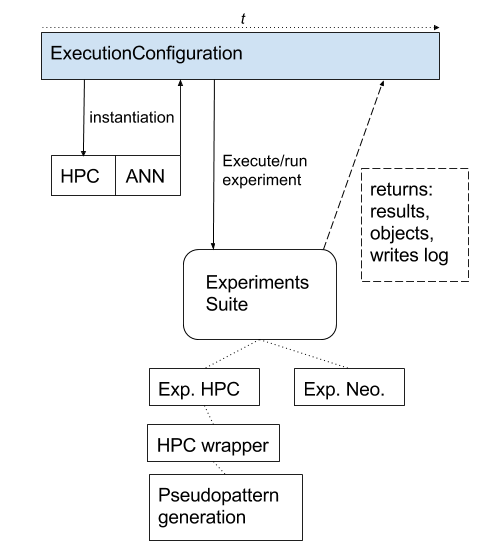
\includegraphics[width=10cm]{fig/ExecutionConfiguration.png}
    \caption{Illustrating the execution and layout of the system containing the dual-network memory model and the experimental environment. First; objects are instantiated containing the two networks of the model, then experiments are run from the experiments suite according to the provided run configuration. This configuration specifies which experiment to run, and with what parameters. Note that the experiment makes calls to the HPC-wrapper, and implements calls to the FFBP ANN, i.e. the neocortical network object/model directly.}
    \label{fig:system_layout}
\end{figure}

In order to generate images of the different layers' activities, simple formulas which generated a rectangular view of a vector of activation values was used, along with the Python Image Library (PIL). Furthermore, in order to save previous results to disk, simple Python file handling was used to write logs, and cPickle was used to store the binary data of objects, enabling later retrieval and analysis of specific hpc-models.

% ====================================== IMPLEMENTATION ===========================================
\section{Implementation}

\subsection{Hippocampal module details}

For the hippocampal network I instantiated shared theano variables, storing the values of vectors for the activation values, and matrices for the weights between the different layers. Topologically, it remains the same as illustrated previously in figure \ref{fig:hattori_2014_model}. In the hippocampal network, the first step of propagating values throughout the model is to simply multiply the activation values of the first layer with the associated weight matrix, representing its connections, storing the result in the subsequent layer; the EC-layer. After this operation, kWTA is performed. For all layers except for the CA3-layer, these operations are simply performed according to the following equations,

\begin{equation}\label{eq:transfer_function_hpc}
    \textbf{x}_j = tanh (\frac{\textbf{x}_i \textbf{W}_{i,j}}{\epsilon}),
\end{equation}

where $\epsilon$ is a steepness parameter. Succeeding this straightforward propagation between the layers, using a common thresholding function, is setting the activation values in a binary fashion according to the k-WTA algorithm;

\begin{equation}
    f(x_i, x_{threshold}) = \begin{cases}
    1, & x_i >= x_{threshold} \\
    0, & otherwise
    \end{cases}
\end{equation}

where $x_{threshold}$ is calculated simply as $x_{threshold} = \frac{x_{k} + x_{k-1}}{2}$, where $x_k$ is the k-th largest activation value in the layer after action potantial potentiation according to equation \ref{eq:transfer_function_hpc}. For pseudocode on the k-WTA implementation, please see Appendix D.
\\

When it comes to the CA3-layer, information is summed from several layers, after which the equations for chaotic neurons are used to attain the next $\eta$-values, which are finally sent through the thresholding function $tanh$ before kWTA is performed according to the firing rate of the layer. The equations, as outlined in chapter \ref{chpt:existing-models} in equations (\ref{hattori_next_output}, \ref{hattori_eta}, \ref{hattori_zeta}), are here given in vector form;

\begin{equation}\label{eq:eta_zeta_sum}
    \textbf{x}(t+1) = f\{ \vec{\eta}(t+1) + \vec{\zeta}(t+1) \}
\end{equation}

\begin{equation}
    \vec{\eta}(t+1) = k_m \vec{\eta}(t) + \sum_{i} \textbf{W}_{i.j} \textbf{x}_i
\end{equation}

\begin{equation}
    \vec{\zeta}(t+1) = k_r \vec{\zeta}(t) - \alpha \textbf{x}_j(t) + \textbf{a}
\end{equation}

where $k_m$ and $k_r$ are a damping factors of refractoriness, $\textbf{x}_j$ is the input values (i.e. former activation values of the CA3-layer), and $\sum_{i} \textbf{W}_{i.j} \textbf{x}_i$ is the sum of all input values from the preceding layers for $i\in\{ec, dg, ca3\}$, and,

\begin{center}
\begin{math}
    \textbf{x}_i = \textbf{x}_{ec} \textbf{W}_{ec, ca3} + \textbf{x}_{dg} \textbf{W}_{dg, ca3} + \textbf{x}_{ec} \textbf{W}_{ca3, ca3}
\end{math}
\end{center}

Having shared variables store the current values for the eta- and zeta-vectors provides a sufficient basis for iterating through time-steps for the chaotic neurons, given that the surrounding activation value vectors and weight matrices also are instantiated. By using Theano, the above definitions of the equations translates more or less directly to symbolic definitions in Theano, thus implementing the model. Please see Appendix D for an excerpt of the hippocampal module, including other code examples, as well as an architectural code overview, and a link to a public git repository containing the full code.

\begin{figure}
    \centering
    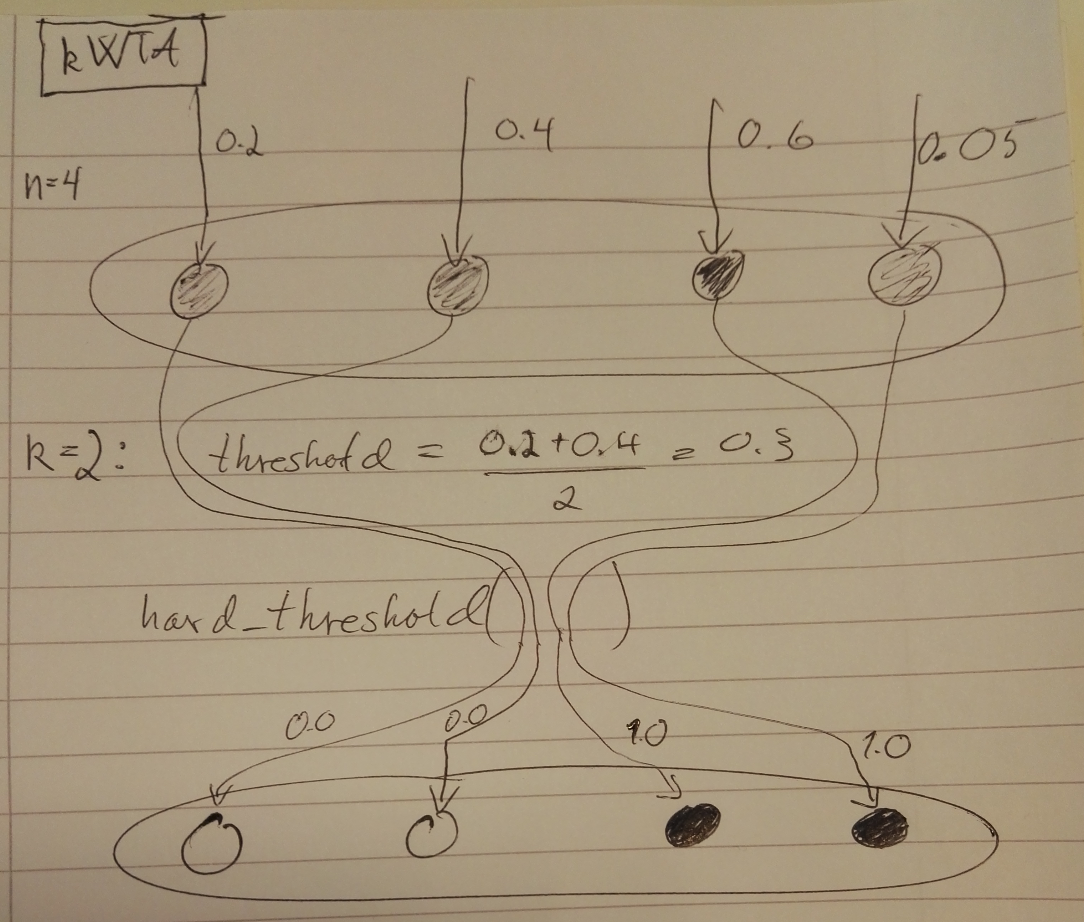
\includegraphics[width=10cm]{fig/kWTA_network_layout}
    \caption{Illustrating kWTA for an arbitrary network layer of size $n=4$. Note that the figure depicts information flowing to  the same layer after binary thresholding has been performed.}
    \label{fig:kWTA_illustration}
\end{figure}

\begin{figure}
    \centering
    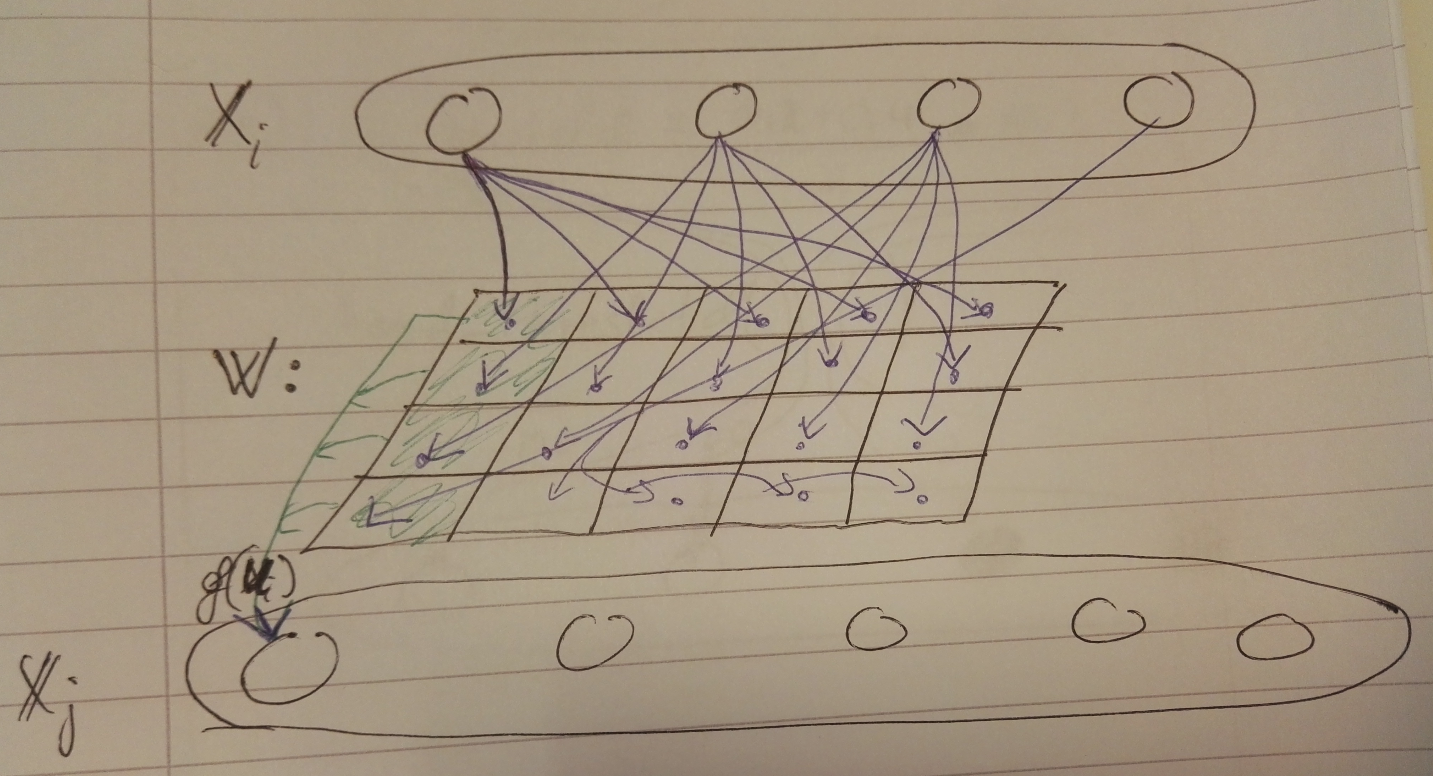
\includegraphics[width=12cm]{fig/network_layout}
    \caption{Illustrating two network layers and the associated weight matrix}
    \label{fig:network_layout}
\end{figure}


\subsection{Neocortical module details}

When it comes to the neocortical module, this is implemented essentially as a traditional back-propagation network; having an input and output-layer, and one hidden layer, along with two weight matrices for the connections between the layers. The L2-norm was used as error-function, and diracs delta function was used to chain the error-signal during back-propagation for an efficient execution, using the gradients starting at the output-layer. While the reader may consult Appendix A for the mathematical details and derivation of the equations associated with the traditional feed-forward back-propagation artificial neural network, the main equations are also given here, being the following,

\begin{equation}
    \Delta \omega_{i,j} = -\alpha \frac{\partial \textbf{E}}{\partial \omega_{i,j}},
\end{equation}

\noindent
which minimizes the error loss-function \textbf{E} w.r.t. the partial derivative of the weight $\omega_{i,j}$ from neuron $i$ to neuron $j$.
In its full form, the term for the derivative of the error loss-function may be written using the chain rule as,

\begin{equation}
    \frac{\partial \textbf{E}}{\partial u_j}\frac{\partial u_j}{\partial \theta_j} = 
    (\sum_{l \in L}\frac{\textbf{E}}{\partial u_l}\frac{\partial u_l}{\partial \theta_l}) f(\theta_j)(1-f(\theta_j),
\end{equation}

\noindent
where $u_j$ is the activation value of node $j$, and $\theta_j$ is neuron $j$'s total input. Starting at the output layer, one may simplify the equation to,

\begin{center}
\begin{math}
    \frac{\partial \textbf{E}}{\partial u_l} \frac{\partial u_l}{\partial \theta_l} \omega_{j,l} = 
    u_l (u_l - d_l) \omega_{j,l},
\end{math}
\end{center}

which may then be used in the preceding layers after updating the subsequent values, as these will then embed the former terms of the chain into the updates. This allows for a simple implementation and a very efficient algorithm/model. Acquisition of a weight-configuration may also be performed on the GPU - however this is regarded as unnecessary in the current paradigm, as the data set and number of iterations remain very small.


% ========================================== PARAMETERS ================================================
\subsection{Model decisions}

During the implementation of the model, I encountered some model aspects that were not clearly stated in the papers on which I base the model; \citep{Hattori2014, Hattori2010}. To proceed with the implementation, certain decisions had to be made. I re-visited the papers' references, as well as the background literature, for consultation on the model details and parametrization. 
My implementation diverges from that of \citep{Hattori2014} in that updating of neuronal values in the CA3-layer occurs synchronously, as opposed to asynchronously in \citeauthor{Hattori2014}'s (\citeyear{Hattori2014}) model.
Asynchronicity may introduce more randomness into a search in dynamic networks, and other algorithms such as cellular automatas or Boltzmann machines \citep{Bar-yam1997}. Thus having the CA3 neurons update their values asynchronously may enable the layer as an auto-associative network to traverse more of its search space - i.e. it is not as limited in what values that the neurons will take after a certain update/propagation from the preceding layers. This may possibly result in being able to recall more patterns within the hippocampal model, but may on the other hand introduce more noise during learning. Thus the question remains whether the benefit during the search and recall outweighs the possible downsides during learning. Because the extra 'wiggle' is in fact present during learning as well, chances are that having an asynchronous updating scheme is more effective. 
The justification of having a synchronized layer updating scheme in the model is that it is a far more efficient implementation - enabling for instance the exploitation of hardware parallelism for matrix operations. Initial experiments of the next chapter (\ref{chpt:experiments}) test and discuss whether asynchronous updating should be part of the model.
\\

As for calculating the next activation values of the chaotic neurons in the CA3-layer the paper of \cite{Hattori2014} did not specify whether to sum the vector and matrix products. Therefore I consulted other references such as \citep{Wakagi2008}, granting insights into and underlining important topological decisions such as the inclusion of the DG-layer during learning, which enables pattern separation. During preliminary experiments, however, it was observed that only including the layer during learning did not result in sufficiently reducing the pattern overlap.
In their work on complementary learning systems, \cite{Norman2003} implement a complementary learning systems containing a hippocampal model which uses expansion encoding in their DG-layer. Arguing that the DG physiologically speaking seems to have the ability to heavily influence the firing patterns of CA3, I therefore implemented a variable weighting of the DG-firing pattern integration on the CA3-layer. Initial experiments showed that a weighting approximately similar to theirs, i.e. about 25 times stronger connections between the DG- and CA3-layer yielded better recall and quicker convergence in the attained model. This suggests that pattern separation may be performed by the DG-layer, and confirms the hypothesis that it may be more strongly interconnected with the CA3-layer.

Regarding the implementation of eta- and zeta-functions in CA3, the thresholding is performed after the sum of the activation value vectors and weight matrices product calculations. In other words, the tangent hypabolicus transfer function is applied to the sum of the eta- and zeta-functions: 

\begin{center}
\begin{math}
    \textbf{x}_{ca3}(t+1) = tanh(\frac{\eta(t+1) + \zeta(t+1)}{\epsilon})
\end{math}
\end{center}

Lastly, it may be argued that a type of recall ... internally, CA3, blabla. However, only once.


\textbf{Notes}

Where should the focus be? \textit{pseudopattern generation and memory consolidation}

HPC module - high-quality pattern extraction, STM with sufficiently high degradation of old memories to avoid dilution and spurious memories

neocortical module - pattern acquisition, acquisition of functional mapping

Analyzation - see notes.
\\

Choices I have made in the implementation that remain unclear in the paper.

Enforce sparsity through weight updates corresponding only to the winners of kWTA - didn't work.

(Alternatively: Through initializing synapses only for a given (local) percentage of neurons. - haven't tried, doesn't make sense since the above didn't work?)

negative weights will necessarily allow for more categorization, and possibly avoiding learning the mean feature vector. However, it reduces perfect recall rates (p. 74) - this may affect especially heteroassociation.